\section{Aufbereitung der Bilder}
\label{scale_Algos}
Für die Gesichtsanalyse wird OpenFace verwendet, dieses Verfahren arbeitet laut Angabe im Paper \cite{OpenFace} am besten auf Gesichtern mit einer Mindestgröße von 100 Pixel, daher werden die Bildbereiche auf diese Größe gebracht. Dies ist notwendig, da die Berechnung meist auf recht kleinen Bildausschnitten ausgeführt werden muss.\\
Dabei ist es wichtig, dass die Gesichtsmerkmale möglichst gut rekonstruiert werden, um die entsprechenden Landmarks zu bestimmen, dabei erhöht sich der Informationsgehalt der Bilder nicht, sie sind nur besser nutzbar, da sie dem Trainingsdatensatz stärker ähneln.\\
Für die \autoref{img_Bicubic} bis \ref{img_NN} wurde die Abbildung von Lena mit einer Kantenlänge von 100 Pixel und ein Schachbrettmuster mit 48 Pixel verwendet und auf eine Größe mit den angegeben Verfahren auf 512 Pixel gebracht. Um den Unterschied zwischen der vergrößerten Lena-Darstellung und der Originalen zu zeigen, wurde das Differenzbild ebenfalls dargestellt.\\
Wird ein Bild vergrößert, müssen weitere Pixel dem Bild hinzugefügt werden. Zur Bestimmung des Farbwertes des Pixels gibt es verschiedene Verfahren, ein Teil wurde ausgewählt und ihre Auswirkung im folgenden getestet.
\subsection{Bicubic-Skalierung}
Der Farbwerte eines Pixel wird ermittelt, indem die umliegenden $4\times 4$ Pixelwerte betrachtet werden um den Farbverlauf als eine Funktion 3. Grades zu bestimmen. Somit werden feinere Details besser dargestellt als beim linearen Verfahren und Kanten bleiben eher erhalten. Allerdings kann es durch den bestimmten Verlauf auch zum Überschwingen kommen, wodurch Fehlfarben entstehen können. Ein Beispiel als Ergebnis dieses Verfahrens ist in \autoref{img_Bicubic} zu sehen. \cite{wiki_Bicubic}
\subsection{Lanczos-Skalierung}
Dieser Filter basiert auf einem bewerteten Durchschnitt der umliegenden Pixel um den neuen Pixelwert zu erhalten. Die Bewertung der einzelnen Pixel wird durch eine Sinc-Funktion bestimmt, damit weiter entferntere Pixel schwächer bewertet werden als näher liegende, siehe \autoref{img_Lanczos}.
\[ L(x)= \left\{ \begin{array}{ll}
\frac{\sin(\pi x)}{\pi x} \cdot \frac{\sin(\pi \frac{x}{a})}{\pi \frac{x}{a}} & \textrm{wenn } -a < x <a, a\ne 0\\
1 & \textrm{wenn } x = 0\\
0 & \textrm{sonst}
\end{array}\right. \]
Außerdem wird durch den Kurvenverlauf der Bewertungsfunktion eine gewisse Bildschärfe erreicht. Die Funktion kann und wird für die Anwendung auf einen $8\times 8$ Pixel großen Bereich begrenzt. \cite{wiki_Lanczos}
\subsection{Linear-Skalierung}
Um den neuen Farbwert zu ermitteln, wird zwischen den nächstgelegenen umliegenden Pixel linear interpoliert, wodurch weitere Farbwerte entstehen. Das Ergebnis ist gleichmäßiger als Nearest-Neighbor, und dennoch ein recht einfaches Verfahren. Die Kanten wirken allerdings unscharf, siehe \autoref{img_Linear}.
\subsection{Nearest-Neighbor-Skalierung}
Dieses Verfahren verwendet als neuen Farbwert den gleichen Wert wie das nächstgelegene Pixel. Dadurch werden nur die ehemaligen Pixel größer und das Gesicht wirkt sehr kantig, da keine neuen Farbwerte bestimmt werden, siehe \autoref{img_NN}. Bei der Vergrößerung des Schachbretts sind keine Farbfehler aufgetreten, da nur zwei Farben vorhanden und diese positionsabhängig sind.
\begin{figure}[p]
	\centering
	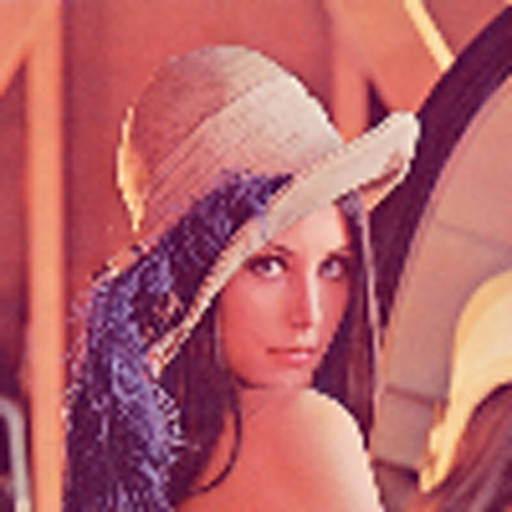
\includegraphics[width=0.24\linewidth]{img/lena100_CUBIC}
	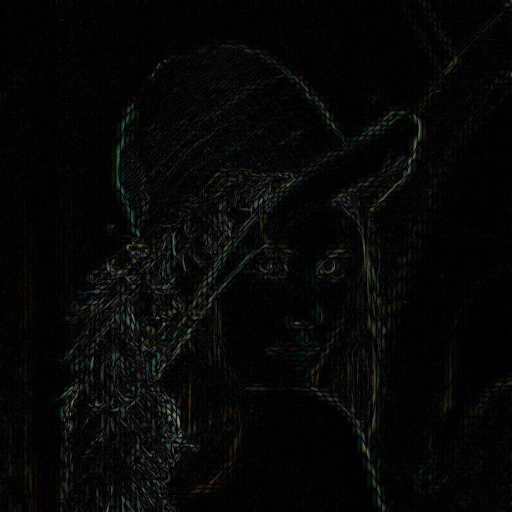
\includegraphics[width=0.24\linewidth]{img/lena100_CUBIC_differenz}
	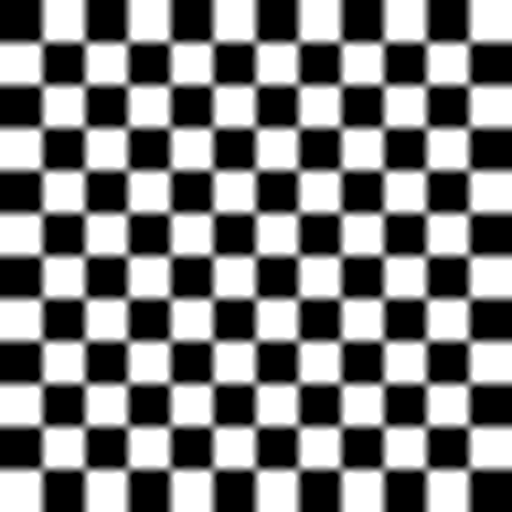
\includegraphics[width=0.24\linewidth]{img/Schachbrett_CUBIC}
	\caption{Vergrößerung der Bilder mittels bikubischem Verfahren.\\
		Links: Lena, Mitte; Differenz zum Original, Recht: Schachbrett}
	\label{img_Bicubic}
\end{figure}
\begin{figure}[p]
	\centering
	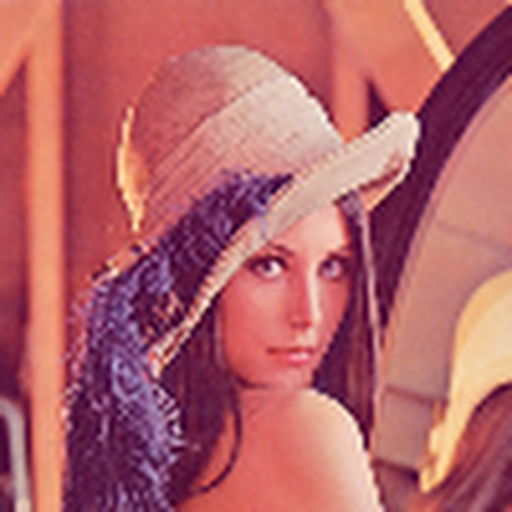
\includegraphics[width=0.24\linewidth]{img/lena100_LANCZOS4}
	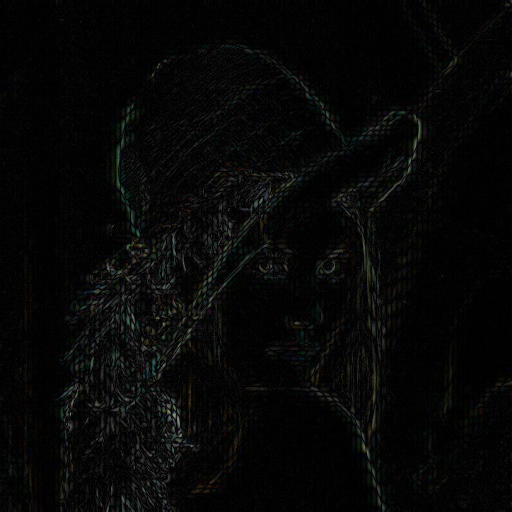
\includegraphics[width=0.24\linewidth]{img/lena100_LANCZOS4_differenz}
	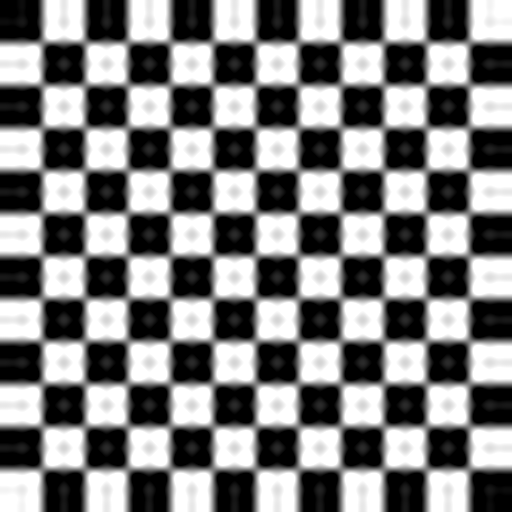
\includegraphics[width=0.24\linewidth]{img/Schachbrett_LANCZOS4}
	\caption{Vergrößerung der Bilder mittels Lanczus-Verfahren.\\
		Links: Lena, Mitte; Differenz zum Original, Recht: Schachbrett}
	\label{img_Lanczos}
\end{figure}
\begin{figure}[p]
	\centering
	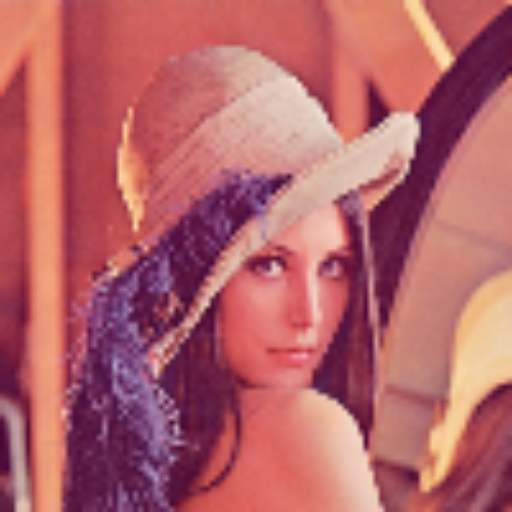
\includegraphics[width=0.24\linewidth]{img/lena100_LINEAR}
	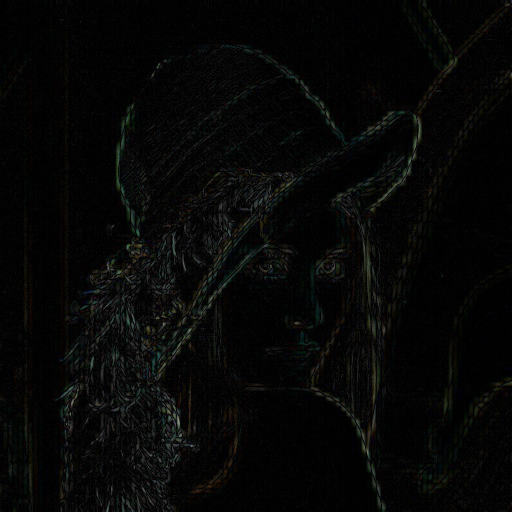
\includegraphics[width=0.24\linewidth]{img/lena100_LINEAR_differenz}
	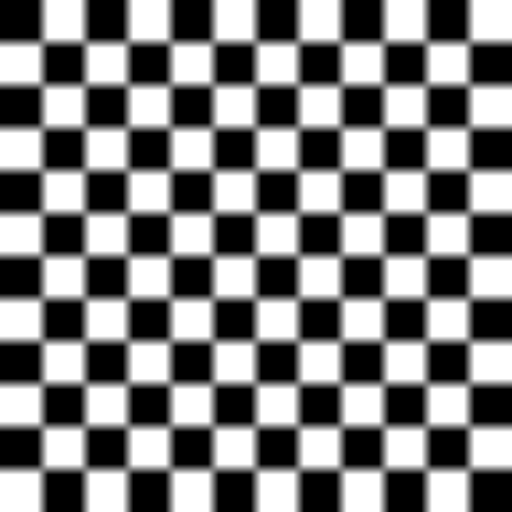
\includegraphics[width=0.24\linewidth]{img/Schachbrett_LINEAR}
	\caption{Vergrößerung der Bilder mittels linearer Interpolation.\\
		Links: Lena, Mitte; Differenz zum Original, Recht: Schachbrett}
	\label{img_Linear}
\end{figure}
\begin{figure}[p]
	\centering
	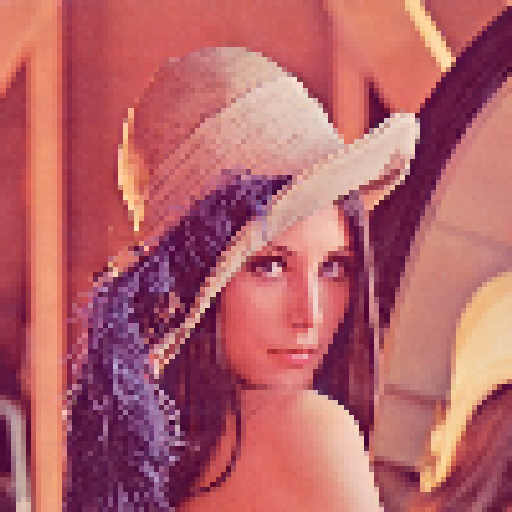
\includegraphics[width=0.24\linewidth]{img/lena100_NN}
	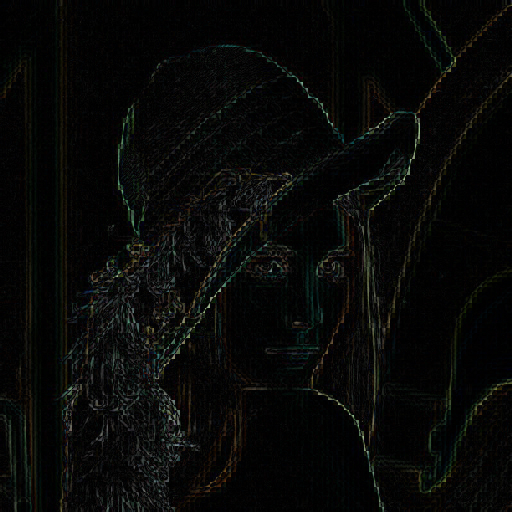
\includegraphics[width=0.24\linewidth]{img/lena100_NN_differenz}
	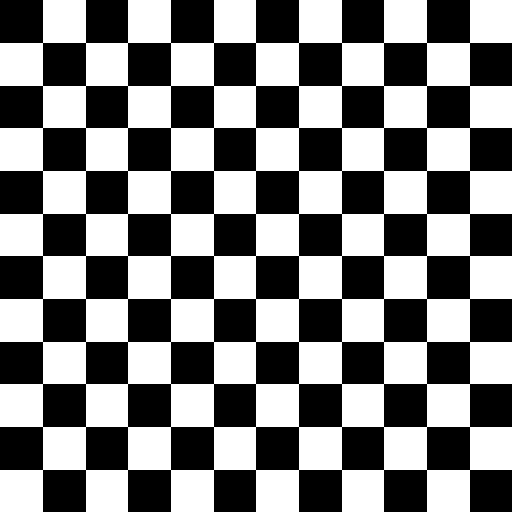
\includegraphics[width=0.24\linewidth]{img/Schachbrett_NN}
	\caption{Vergrößerung der Bilder mittels Nearest-Neighbor.\\
		Links: Lena, Mitte; Differenz zum Original, Recht: Schachbrett}
	\label{img_NN}
\end{figure}
